% !TEX root = ../main.tex
\fancychapter{Solution}%
\label{chap:solution}
\cleardoublepage{}

\todo[inline]{{\bfseries TODO}: Vastly improve on this\ldots}

\noindent
Despite strides in enhancing performance and efficiency of geometric constraint
solving approaches, briefly discussed in \Cref{sec:intro.constraints}, the core
issue lies in the generality of geometric constraint solvers.  Although several
approaches employ efficient methods to find a solution, they resort to solving
potentially well-known problems generically when computationally lighter
solutions exist.  Instead of delegating the problem to a solver, a more
efficient approach would be to pinpoint the type of geometric constraint itself,
specializing a solution for several applicable entities.  Take the tangency
constraint as an example: positioning two circles tangent to each other or a
line tangent to an ellipse.  Depending on the inputs, these constraints might
have particularly efficient solutions for each case, in kind making the
computation more efficient.

Classical numerical methods constitute alluring alternatives to the predominant
graph-based approaches.  Having been studied for several decades, even if the
provided solution does not encompass all the possible values within the
problem's domain, they can be used to target specific problems efficiently.
Nonetheless, these suffer from robustness issues discussed in
\cref{sec:related.robustness}, effectively yielding inaccurate solutions if
precautions aren't taken.  A similar argument can be made about algebraic
methods.

This work aims to implement a series of geometric constraint primitives in an
already expressive \ac{TPL} to overcome the need for the specification of
unnecessary details when modeling geometrically constrained entities, promoting
an easier and more efficient usage.  Choosing to implement these in a \ac{TPL}
further avoids the code complexity that arises from what could be analogous
specifications in a \ac{VPL}, a subject previously discussed in
\cref{sec:intro.ad}.

Moreover, by relying on an exact geometry computation library, one of the core
features of this solution lies in the capability of transparently dealing with
the previously addressed robustness issues.  The user can then resort to these
primitives, and, by composing them, elegantly specify the set of geometric
constraints necessary in order to produce the idealized model.  Since the
available primitives will implement specialized solutions for a finite set of
shapes the user can utilize in whichever combination possible during the design
process, the solution will be exempt of a generic solver component, potentially
boosting performance of design generation.

\Cref{fig:solution.arch} shows the typical \ac{AD} workflow and how the proposed
solution could be integrated with the \ac{AD} tool.  The encapsulated modules in
the figure represent the underlying computation library as an external
component, featuring the geometric constraint primitives library and the code
wrapping the computation library.

\begin{figure}[htbp]
  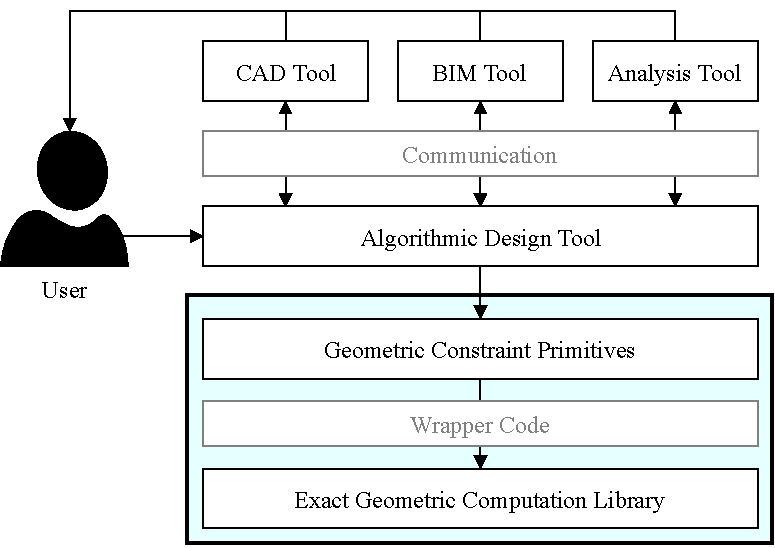
\includegraphics[width=\textwidth]{fig/solution-arch}
  \caption[Solution architecture within \acs{AD} workflow]{
    General overview of the solution's architecture encapsulated within the
    blue colored box beneath a depiction of the typical \ac{AD} workflow.}%
  \label{fig:solution.arch}
\end{figure}
